\documentclass{article}

\title{Conception du microprocesseur}
\date{13/12/2021}
\author{Florian Tousnakhoff \and Fabio d'Ortoli Galerneau \and Félix Lebrat}

\usepackage{moreverb}
\usepackage[top=2cm]{geometry}
\usepackage{bbm}
\usepackage{amsfonts}
\usepackage{amsmath}
\usepackage{amssymb}
\usepackage{bbold}
\usepackage{amsthm}
\usepackage{pdfpages}
\usepackage{graphicx}
\usepackage{multicol}

\renewcommand{\thesection}{}

\begin{document}
    \maketitle
    \section{Architecture générale}

    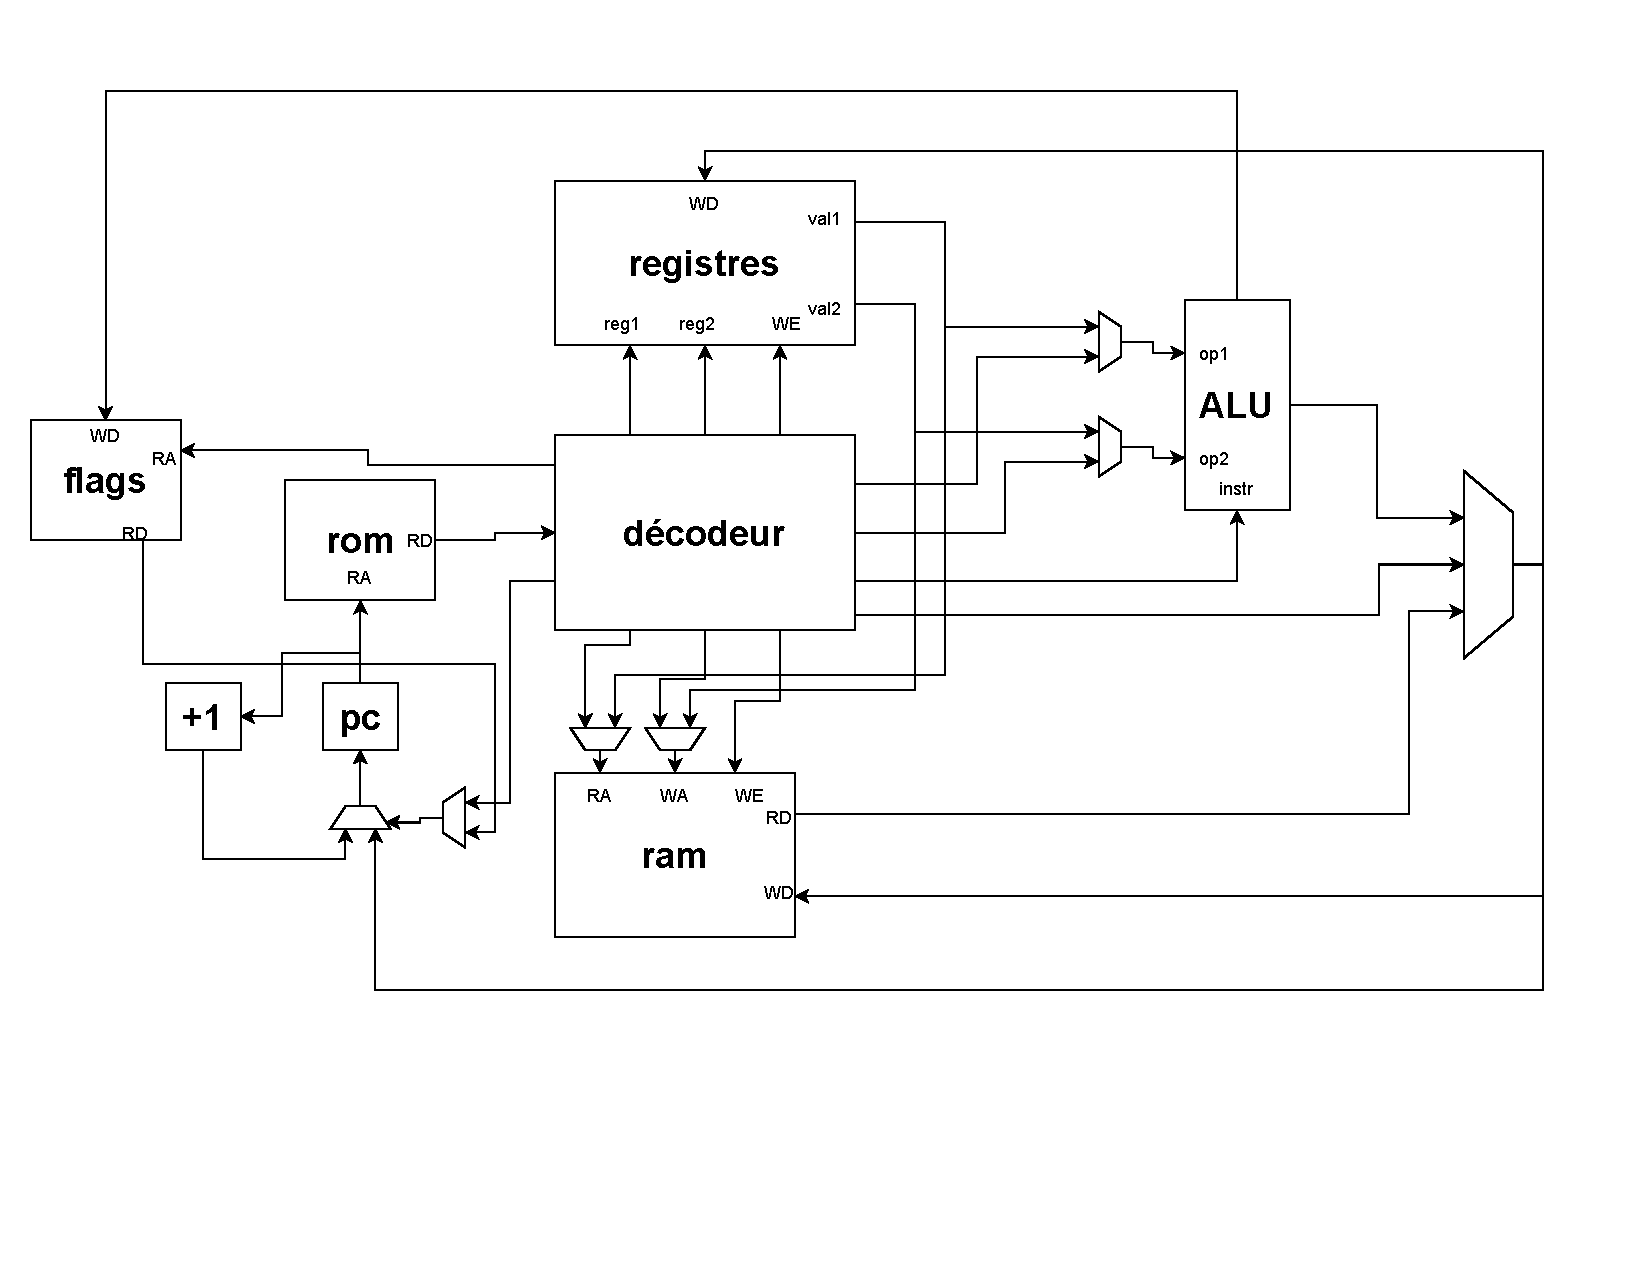
\includegraphics[width=17.8cm,height=12.6cm,page=1]{schema.pdf}
    \begin{itemize}
        \item RA : read address
        \item WE : write enable
        \item WA : write address
        \item RD : read data
        \item WD : write data
    \end{itemize}
    les multiplexeurs dont l'entrée de contrôle n'est pas précisée sont
    contrôlés par le décodeur

    \section{Registres}
    Le microprocesseur contient 16 registres généraux de 32 bits :
    \begin{multicols}{2}
     \begin{itemize}
        \item rax
        \item rbx
        \item rcx
        \item rdx
        \item rsi
        \item rdi
        \item rbp
        \item rsp
        \item r8
        \item r9
        \item r10
        \item r11
        \item r12
        \item r13
        \item r14
        \item r15
    \end{itemize}
    \end{multicols}
    qui sont donc adressés sur 4 bits

    \section{RAM}
    L'adressage de la RAM se fait sur 16 bits,
    et la taille des mots est de 32 bits.

    \section{ALU}
    L'ALU prends deux entrées sur 32 bits et sort le résultat, sur 32 bits également, de l'opération spécifiée
    par l'entrée \texttt{instr} sur 3 bits selon le code suivant :
    \begin{multicols}{2}
    \begin{enumerate}
        \item non bit à bit
        \item et bit à bit
        \item ou bit à bit
        \item ou exclusif bit à bit
        \item multiplication
        \item addition
        \item soustraction
    \end{enumerate}
    \end{multicols}
    et définit les drapeaux \texttt{neg} et \texttt{null} en fontion du résultat.

    \section{Instructions}
    Les instructions sont codées sur 32 bits, dont 6 pour l'opcode et 13 par opérande. Elles sont stockées dans une
    ROM, adressée sur 16 bits, et lues par le décodeur. Le jeu d'instructions est le suivant :
    \begin{multicols}{2}
        \begin{itemize}
            \item MOV op1 op2
            \item NOT op
            \item XOR op1 op2
            \item OR op1 op2
            \item AND op1 op2
            \item ADD op1 op2
            \item SUB op1 op2
            \item MUL op1 op2
            \item LSL op
            \item LSR op
            \item CMP op1 op2 (définit les drapeaux pour op2-op1)
            \item JMP op
            \item JZ op (jump if null)
            \item JNZ op (jump if not zero)
						\item JL op (jump if less than)
        \end{itemize}
    \end{multicols}
    \paragraph{Modes d'adressage :}
    \begin{itemize}
        \item MOV : op1 peut être une constante, une adresse RAM
ou un registre, et op2 peut être une adresse RAM ou un registre.
        \item Pour les opérations arithmétiques ou logiques à une opérande, op doit être un registre
        \item Pour les opérations arithmétiques ou logiques à deux opérandes, op1 doit être une constante ou un registre
et op2 un registre.
        \item CMP : op1 et op2 sont des constantes ou des registres
        \item pour les instructions de branchement, op est une constante ou un registre
    \end{itemize}

    \section{Choix techniques :}
    Les netlists sont écrites directement, à l'aide du C++ (ou d'un autre langage).
		\section{Génération de netlist en C++}
		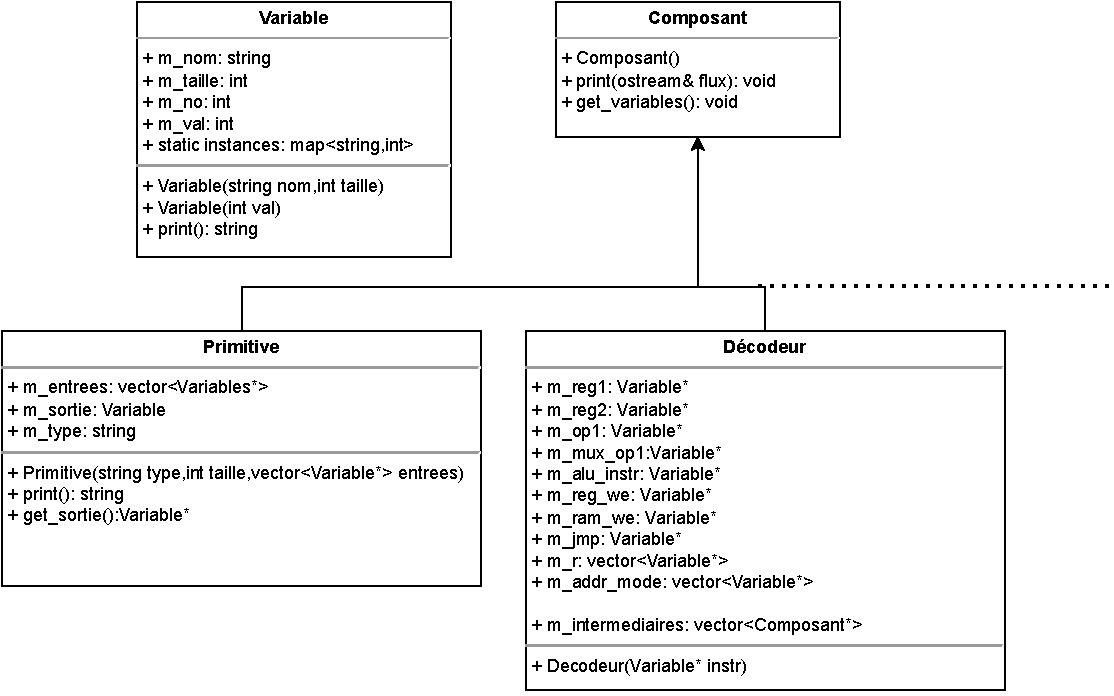
\includegraphics[width=14.8cm,height=10.6cm,page=1]{uml.pdf}\\
		Le dictionnaire \texttt{instances} dans la classe \texttt{Variable} associe un nom de variable au nombre de variables portant ce nom. Lorsqu'une variable est créée, on peut donc lui associer un numéro pour éviter la duplication des noms. Une netlist est représentée par un ensemble de \texttt{Composant}. Tous les \texttt{Composant} ont des méthodes \texttt{get\_variables} et \texttt{print}. La première renvoit l'ensemble des variables déclarées dans le \texttt{Composant} et la deuxième sert à écrire les équations qui les définissent dans un flux. De manière générale, les entrées et les sorties des composants sont représentées par des \texttt{Variable}.
		\newpage
		\section{Schéma du gestionnaire de registres}
		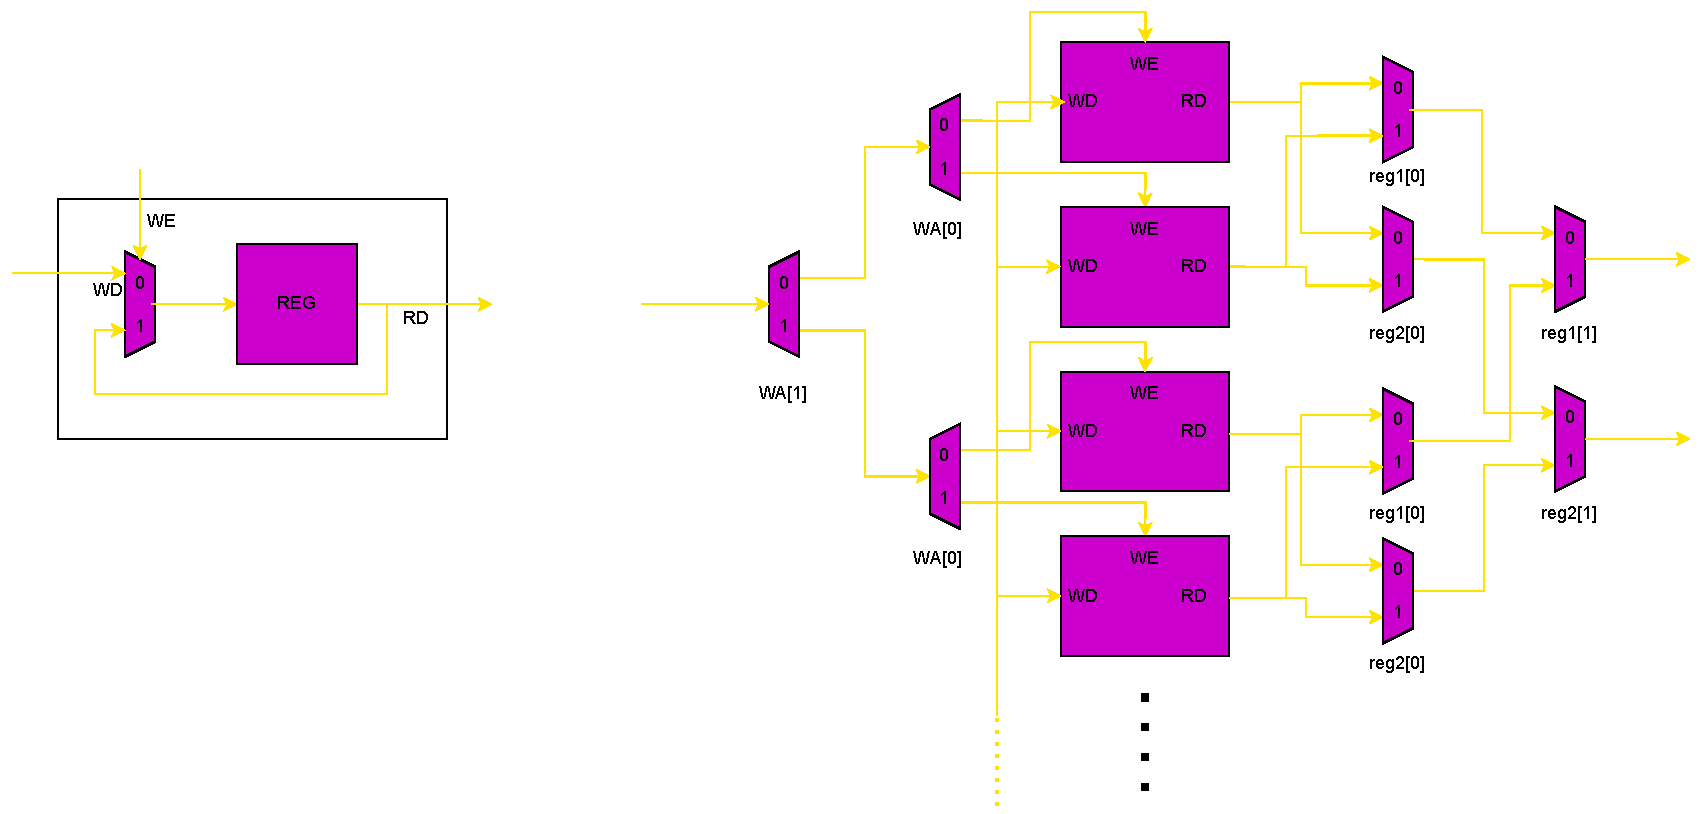
\includegraphics[width=14.8cm,height=10.6cm,page=1]{gestionnaire_registres.pdf}
		\newpage
		\section{Schéma de l'ALU :}
		\includegraphics[scale=0.75]{ual.png}
		\newpage
		\section{Assembleur et Horloge:}
		L'assembleur a été réalisé en OCaml, il consiste en un lexer, un parser et une fonction transformant l'arbre de syntaxe abstraite en code binaire lu et reconnu par le décodeur du microprocesseur.\\	
		L'Horloge a été faite avec l'assembleur, elle donne l'heure du Méridien de Greenwich.\\
		Le signal d'horloge du microprocesseur est donné par le timestamp (nombre de secondes depuis le premier janvier 1970) et est transformé par le programme en la date.\\
		Cela est ensuite mis en mémoire et on fait pointer le registre r14 vers cet endroit de la mémoire qui sera ensuite affiché par l'afficheur 7 segments.\\
\end{document}
